\documentclass[9pt,twocolumn,twoside,]{pinp}

%% Some pieces required from the pandoc template
\providecommand{\tightlist}{%
  \setlength{\itemsep}{0pt}\setlength{\parskip}{0pt}}

% Use the lineno option to display guide line numbers if required.
% Note that the use of elements such as single-column equations
% may affect the guide line number alignment.

\usepackage[T1]{fontenc}
\usepackage[utf8]{inputenc}

% pinp change: the geometry package layout settings need to be set here, not in pinp.cls
\geometry{layoutsize={0.95588\paperwidth,0.98864\paperheight},%
  layouthoffset=0.02206\paperwidth, layoutvoffset=0.00568\paperheight}

\definecolor{pinpblue}{HTML}{185FAF}  % imagecolorpicker on blue for new R logo
\definecolor{pnasbluetext}{RGB}{0,101,165} % default in pinp.cls



\title{Factors Influencing Student Performance in Mathematics}

\author[The University of Sydney]{Hongjie Deng, Anan Wang, Yi Wang,
Ranran Zhang, Jingyi Wu}


\setcounter{secnumdepth}{5}

% Please give the surname of the lead author for the running footer
\leadauthor{}

% Keywords are not mandatory, but authors are strongly encouraged to provide them. If provided, please include two to five keywords, separated by the pipe symbol, e.g:
 \keywords{  education |  linear regression |  student
performance |  UCI dataset  }  

\begin{abstract}

\end{abstract}

\dates{This version was compiled on \today} 


% initially we use doi so keep for backwards compatibility
% new name is doi_footer


\begin{document}

% Optional adjustment to line up main text (after abstract) of first page with line numbers, when using both lineno and twocolumn options.
% You should only change this length when you've finalised the article contents.
\verticaladjustment{-2pt}

\maketitle
\thispagestyle{firststyle}
\ifthenelse{\boolean{shortarticle}}{\ifthenelse{\boolean{singlecolumn}}{\abscontentformatted}{\abscontent}}{}

% If your first paragraph (i.e. with the \dropcap) contains a list environment (quote, quotation, theorem, definition, enumerate, itemize...), the line after the list may have some extra indentation. If this is the case, add \parshape=0 to the end of the list environment.


\section{Abstract}\label{abstract}

This report explores the key determinants of students' final Mathematics
grade (G3) using the UCI Student Performance (Math) dataset. After
exploratory analysis and feature selection, we built and compared
several linear models addressing multicollinearity and transformation
needs. The final model explained 62\% of the variance, with prior
achievement ((G1+G2)/2) emerging as the dominant predictor. A
complementary logistic model confirmed that stronger prior grades and
supportive family backgrounds increase the probability of scoring above
10.

\section{Introduction}\label{introduction}

In 2006, around 40\% of young people in Portugal left school
early---twice the average of the European Union---showing alarming
trends in student achievement and engagement. This study baseline
attempts to understand what really impacts the academic achievement of
students in key subjects. Through the study of the learning environment,
family and personal factors, the study attempts to understand what
impacts students' academic performance to the highest degree. This
should give actionable intelligence to educators and policymakers aimed
at performance improvement and dropout rate reduction.In the report, all
the data are sourced from Portuguese high schools.

\section{Dataset}\label{dataset}

For the analysis, the more objective measure of academic ability within
the datasets, the \textbf{Mathematics dataset}, was used rather than the
\textbf{Portuguese language dataset}, which is more influenced by
culture and language.

This dataset has 395 observations and 33 variables, 16 of which are
numerical and 17 categorical, and no missing variables according to the
official source.

Data was collected from Portuguese secondary school students and
consisted, among other things, of demographics, family and social
background, study habits, and behaviors in school. These variables
provide a solid demographic and social foundation to study the
constellation of social, personal, and academic factors affecting
performance in mathematics.

\subsection{Key variables (used later)}\label{key-variables-used-later}

\begin{itemize}
\tightlist
\item
  \textbf{higher} --- wants to take higher education (binary: yes/no)\\
\item
  \textbf{Mjob} --- mother's job\\
\item
  \textbf{romantic} --- with a romantic relationship (binary: yes/no)\\
\item
  \textbf{goout} --- going out with friends (numeric)\\
\item
  \textbf{Medu} --- mother's education (0--4)\\
\item
  \textbf{G2} --- second period grade (0--20)\\
\item
  \textbf{Walc} --- weekend alcohol consumption\\
\item
  \textbf{famrel} --- quality of family relationships
\end{itemize}

\section{Analysis}\label{analysis}

\subsection{Linear}\label{linear}

To investigate the key academic and demographic factors influencing
students' final grades (G3), several multiple linear regression models
were developed and refined using the student-math dataset. The analysis
followed the standard workflow introduced in class, including initial
model construction, diagnostic checking, model improvement through
transformation and multicollinearity analysis, and final model
validation.

The initial model incorporated all theoretically relevant predictors:

\[G3 \sim higher + Mjob + romantic + G2 + G1 + Medu + Fedu + \]
\[goout + failures + age + absences + Walc + famrel + activities\]

The results indicated that G1 and G2 were strong and statistically
significant positive predictors of the final grade, suggesting that
earlier academic performance plays a dominant role in determining later
achievement. Variables such as age, absences, and family relationship
(famrel) also showed smaller but significant effects. Although the model
achieved a high explanatory power (\(Adjusted R\^2 = 0.83\)), residual
analysis revealed evidence of non-normality and heteroscedasticity,
indicating that key regression assumptions were violated.

To address these issues, a square-root transformation was applied to the
dependent variable. The transformed model exhibited improved residual
normality and variance stability, while maintaining reasonable
explanatory power (Adjusted R\^{}2 ≈ 0.67). The significance and
direction of key predictors remained consistent, confirming that the
transformation enhanced model validity and interpretability with only a
modest reduction in fit.

Further analysis revealed a strong correlation between G1 and G2 (r =
0.85), indicating severe multicollinearity. To mitigate this issue, the
two variables were replaced with their average (G1 + G2)/2, representing
overall early academic performance. The modified model successfully
eliminated multicollinearity, as shown by more stable coefficient
estimates and comparable explanatory power (Adjusted R\^{}2 ≈ 0.62). In
this final form, average prior performance, absences, and famrel were
significant predictors, while age and romantic relationships showed mild
negative effects.

The AIC-based backward stepwise selection confirmed that no redundant
predictors remained, and subsequent 10-fold cross-validation
demonstrated that the final model achieved comparable predictive
accuracy to the previous model while offering greater parsimony and
interpretability. Therefore, the third model was selected as the final
specification, providing the best balance between accuracy, robustness,
and explanatory clarity.

\[\sqrt{G3} \sim higher + Mjob + romantic + (G1 + G2)/2 + Medu + Fedu + \]
\[goout+ failures + age + absences + Walc + famrel + activities\]

\subsection{\texorpdfstring{\textbf{Logistic
model}}{Logistic model}}\label{logistic-model}

We noticed that our linear model failed to meet the linearity,
homoscedasticity , normality assumptions. This motivated us to
complement our linear model with a logistic model to better predict math
final grade. We also considered the extreme lower-tail observations of
G3. Considering the range of G3 is from 0 to 20, we firstly chose the
cutpoint 10 to split the continuous final grade G3 into a binary
variable；this mid-scale threshold aligns with the natural grading
scheme and produces approximately balanced class distributions.
Cross-validation also supported 10 as the best split in terms of overall
RMSE/MAE. We then convert the observations whose G3 \textless= 10 to 0
and observations whose G3 \textgreater{} 10 to 1. We then fit a logistic
regression, with predictors selected from our final linear model. From
the logistic model summary plot, we found that prior grade (average of
G1 and G2) and strongly significant, while weekend alcohol consumption
(Walc) and famrel are also significant at the 5\% level;.Other
behavioral or social variables such as absences, weekend alcohol
consumption, and romantic status show less significant impact. In terms
of the coefficients of significant predictors, we found (G1+G2)/2
increasing one point will increase the G3 \textgreater{} 10 probability
by 36.7\%; Walc increasing one level increases it by 22.1\%; famrel
increasing one level increases it by 36.3\%; age increasing one year
decreases it by 37.6\%. This highlights that prior performance and
family relationship quality are strongly associated with passing,
whereas greater age is associated with a substantially lower probability
of passing.These predictors provide complementary evidence to support
early inferences system development

\section{Result}\label{result}

Among the four candidate models tested through transformation and
cross-validation, Model 3 was selected as the final specification. It
combines G1 and G2 into their average to remove multicollinearity and
provides the best balance between accuracy, interpretability, and
robustness. The model explains about 62 \% of the variance in students'
final mathematics grades (Adjusted R² = 0.62), and the overall F-test (p
\textless{} 2.2 × 10⁻¹⁶) confirms strong statistical significance.

In this model, prior academic performance ((G1 + G2)/2) is the dominant
positive predictor of the final outcome, while parental education and
family relationships show minor positive associations. Factors such as
age, romantic relationship status, and extracurricular activities
exhibit minimal additional explanatory power. Diagnostic checks show
that independence holds, but the residual--fitted plot displays slight
curvature and unequal variance, and the Q--Q plot departs from normality
at both tails. Despite these mild violations, the model performs
consistently across training and validation folds, indicating stable
in-sample and out-of-sample reliability.

\section{Conclusion and discussion}\label{conclusion-and-discussion}

The results consistently indicate that early academic achievement is the
most reliable determinant of students' mathematics performance,
confirming the importance of sustained effort and prior preparation. The
logistic regression further validates these findings by showing that
higher prior scores and positive family support increase the probability
of passing, whereas previous failures and absences reduce it. Together,
both models provide converging evidence that foundational academic
strength and stable support networks drive success more than lifestyle
or demographic variables.

However, several limitations remain. The model focuses mainly on
academic and demographic variables and omits psychological and
motivational factors, restricting its explanatory scope. The uneven
distribution of the dependent variable (G3)---with many zeros---violates
normality assumptions and may distort coefficient accuracy. The
assumption of strict linearity also oversimplifies relationships, as
student performance likely involves nonlinear and interaction effects.
Finally, residual diagnostics show heteroscedasticity and non-normal
errors, suggesting that transformations or nonlinear approaches could
improve model robustness.

Future work should expand the variable set to include behavioural and
attitudinal measures and apply nonlinear or logistic frameworks to
better accommodate zero-heavy outcomes. Overall, the analysis concludes
that consistent prior performance is the clearest and most stable
predictor of mathematics achievement, while broader variable coverage
and flexible modelling would enhance predictive power and
interpretability. \newpage

\section{References}\label{references}

\begingroup
\setlength{\parindent}{0pt}
\setlength{\parskip}{0.5em}
\sloppy
\emergencystretch=2em

\Urlmuskip=0mu plus 2mu \def\UrlBreaks{\do\/\do-\do\_\do\.\do\?\do\&}

\hangindent=0.5in \hangafter=1 Allensworth, E., \& Easton, J. Q. (2007).
\textit{What matters for staying on-track and graduating in Chicago Public High Schools}.
Consortium on Chicago School Research at the University of Chicago.

\par

\hangindent=0.5in \hangafter=1 Keppens, G. (2023). School absenteeism
and academic achievement: Does the timing of the absence matter?
\textit{Learning and Instruction, 86}, Article 101769.

\par

\hangindent=0.5in \hangafter=1 Zhao, L., \& Zhao, W. (2022). Impacts of
family environment on adolescents' academic achievement: The role of
peer interaction quality and educational expectation gap.
\textit{Frontiers in Psychology, 13}.

\par

\hangindent=0.5in \hangafter=1 Centers for Disease Control and
Prevention. (2024, July 19).
\textit{Alcohol behaviors and academic grades}.

\par

\hangindent=0.5in \hangafter=1 Pedersen, T. L., Wickham, H., \& van den
Brand, N. (n.d.).
\textit{ggplot2: Elegant Graphics for Data Analysis (3e)}.
\url{https://ggplot2-book.org/}

\par

\hangindent=0.5in \hangafter=1 Tidyverse. (n.d.).
\url{https://tidyverse.org/}

\par

\hangindent=0.5in \hangafter=1 STHDA. (n.d.).
\textit{ggfortify: Extension to ggplot2 to handle some popular packages}.
\url{https://www.sthda.com/english/wiki/ggfortify-extension-to-ggplot2-to-handle-some-popular-packages-r-software-and-data-visualization}

\par

\hangindent=0.5in \hangafter=1 Kuhn, M. (n.d.).
\textit{A Short Introduction to the caret Package}.
\url{https://cran.r-project.org/web/packages/caret/vignettes/caret.html}

\par

\hangindent=0.5in \hangafter=1 Wickham, H., Fran\c{c}ois, R., Henry, L.,
\& M"uller, K. (n.d.). \textit{A grammar of data manipulation}.
\url{https://dplyr.tidyverse.org/}

\par

\hangindent=0.5in \hangafter=1 UCI Machine Learning Repository. (n.d.).
\textit{Student Performance}.
\url{https://archive.ics.uci.edu/dataset/320/student+performance}

\par

\endgroup

\section{Figures}\label{figures}

\begin{center}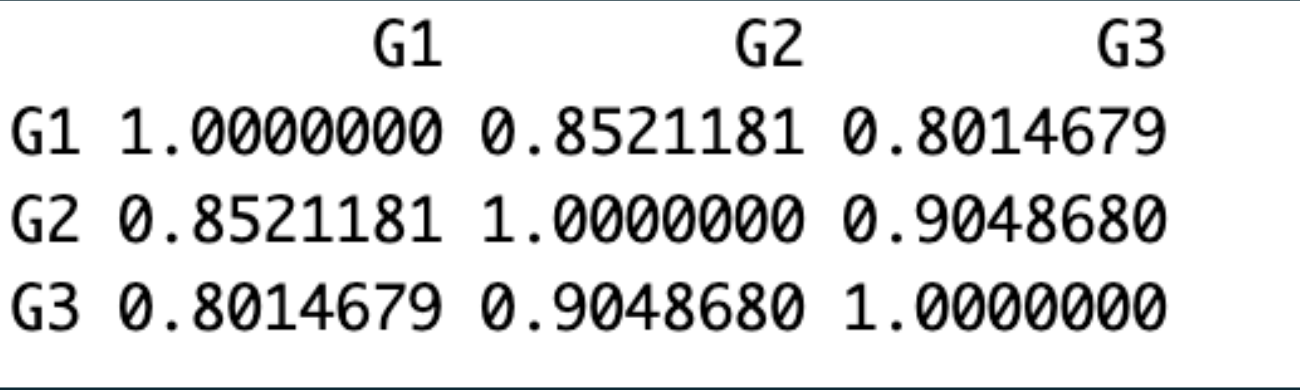
\includegraphics[width=0.7\linewidth]{1} 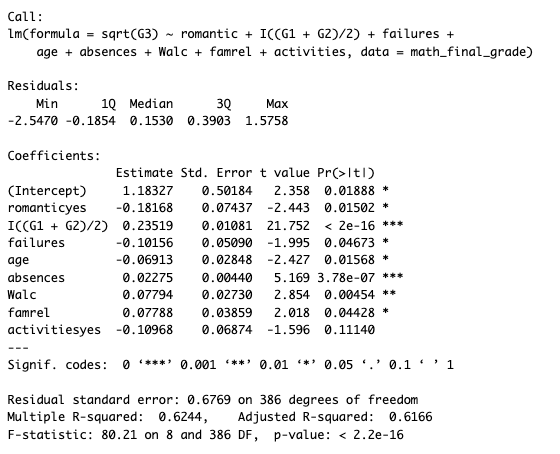
\includegraphics[width=0.7\linewidth]{2} 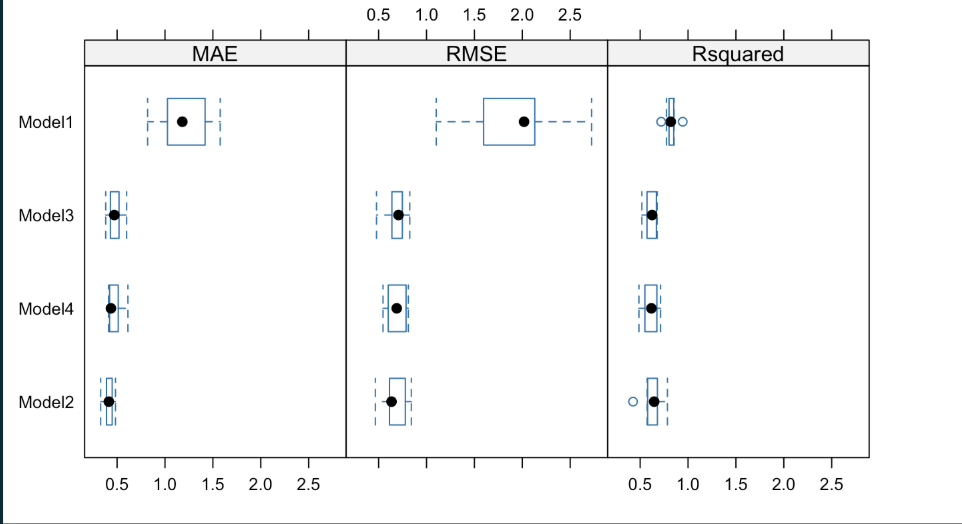
\includegraphics[width=0.7\linewidth]{3} 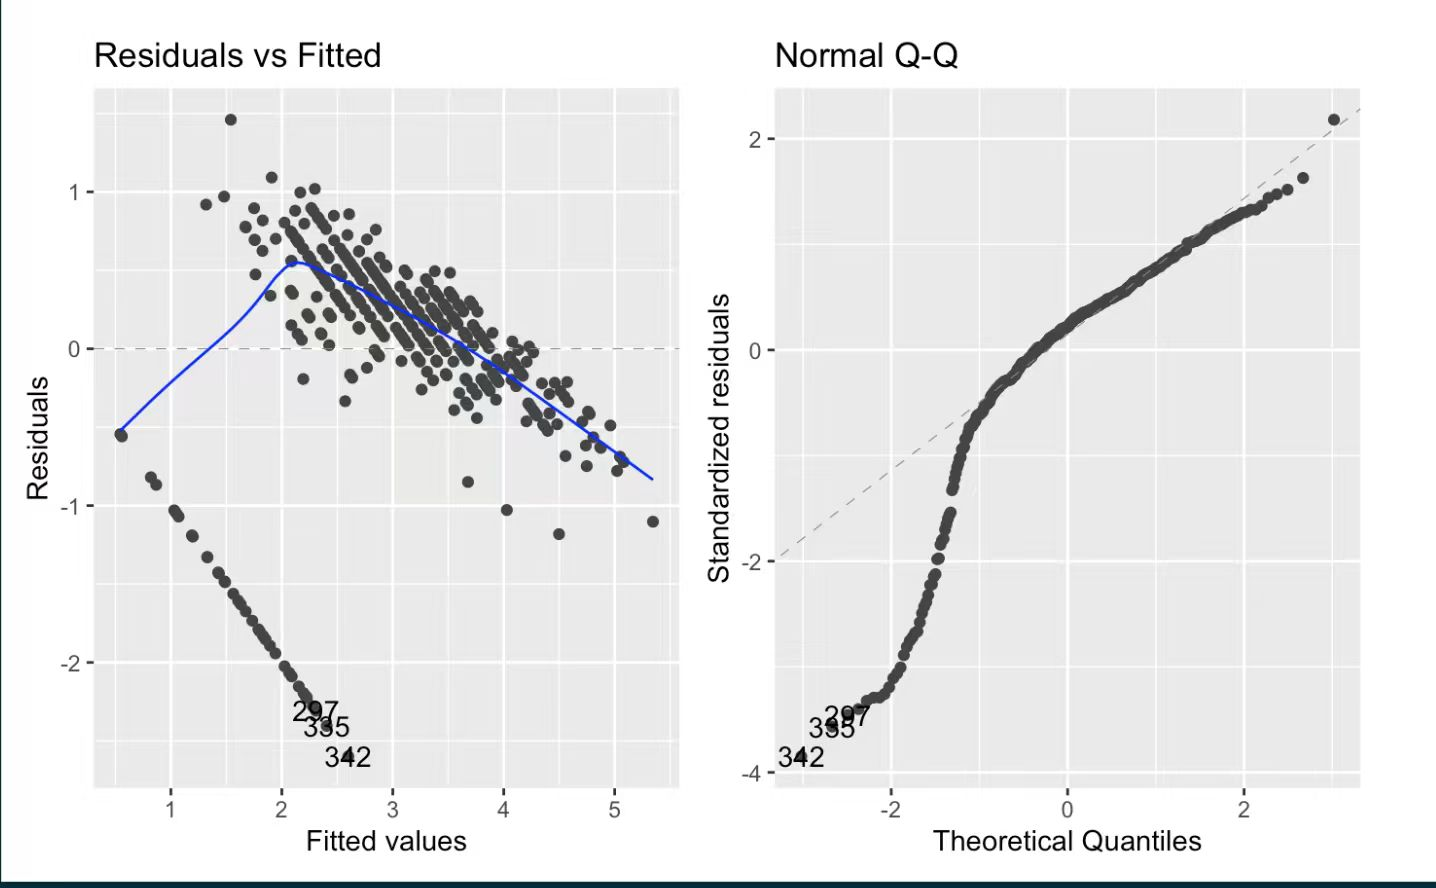
\includegraphics[width=0.7\linewidth]{4} 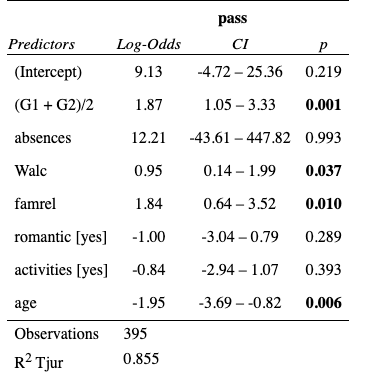
\includegraphics[width=0.7\linewidth]{5} \end{center}

%\showmatmethods

\pnasbreak 

\bibliography{refs.bib}
\bibliographystyle{jss}



\end{document}
